\documentclass[crop,tikz]{standalone}
\usepackage{pgfplots}
\pgfplotsset{compat=1.13}

% Field lines and lines of constant potential for an electric dipole.
%
% Inspired by the expressions given in Fließbach, "Arbeitsbuch zur
% Theoretischen Physik", example 11.7.

\pgfplotsset{
  inverted/.style = {
    every axis legend/.append style={
      draw=white,
      fill=hardblack,
      text=white
    }
  },
  every non boxed x axis/.append style={
    axis line style={-latex}
  },
  every non boxed y axis/.append style={
    axis line style={-latex}
  }
}

\begin{document}

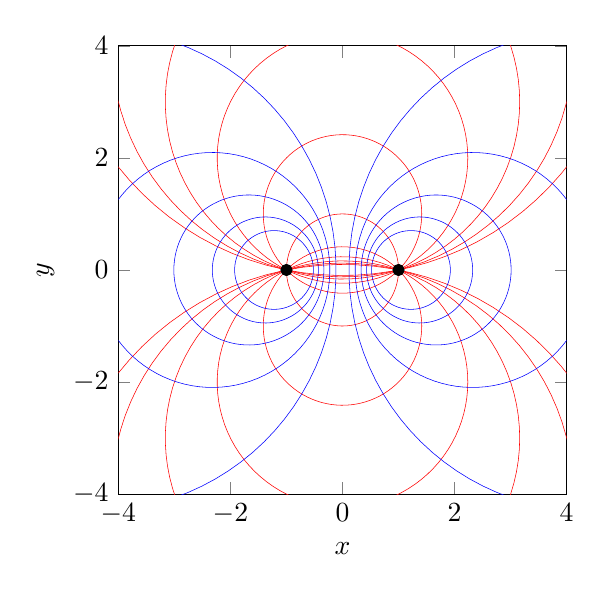
\begin{tikzpicture}
  \pgfmathsetmacro{\numberoffieldlines}{10};
  \pgfmathsetmacro{\numberofpotentiallines}{10};
  \pgfmathsetmacro{\chargepos}{1};
  \pgfmathsetmacro{\remin}{-4};
  \pgfmathsetmacro{\remax}{4};
  \pgfmathsetmacro{\immin}{-4};
  \pgfmathsetmacro{\immax}{4};
  \begin{axis}[
    axis equal image,
    xmin={\remin}, xmax={\remax},
    ymin={\immin}, ymax={\immax},
    xlabel={$x$},
    ylabel={$y$},
    samples=100,
    declare function = {
      phir(\a,\c) = 2*sqrt(\c)*\a/(1 - \c);
      phix(\x,\c,\a,\s) = phir(\a,\c)*cos(x) + \s*(1 + \c)/(1 - \c)*\a;
      phiy(\x,\c,\a) = phir(\a,\c)*sin(x);
      Er(\a,\d) = sqrt(\a^2 + \d^2);
      Ex(\x,\d,\a) = Er(\a,\d)*cos(x);
      Ey(\x,\d,\a) = Er(\a,\d)*sin(x) - \d;
      fc(\n,\nmax) = 1/\nmax*exp(2*\n/\nmax*ln(\nmax));
    },
    ]
    % field lines
    \pgfplotsinvokeforeach{{-\chargepos*\numberoffieldlines/2},...,{\chargepos*\numberoffieldlines/2}}{
      \addplot[red,very thin,domain=0:360] ({Ex(x,#1,\chargepos)},{Ey(x,#1,\chargepos)});
    }
    % lines of constant potential
    \pgfplotsinvokeforeach{0,...,{\numberofpotentiallines}}{
      \addplot[blue,very thin,domain=0:360] ({phix(x,fc(#1,\numberofpotentiallines),\chargepos, 1)},{phiy(x,fc(#1,\numberofpotentiallines),\chargepos)});
    }
    % charges
    \addplot[only marks,mark=*] coordinates { ({ \chargepos},0) };
    \addplot[only marks,mark=*] coordinates { ({-\chargepos},0) };
  \end{axis}
\end{tikzpicture}
\end{document}
